\documentclass{article}
\usepackage{authblk}
\renewcommand{\thefigure}{S\arabic{figure}}

\title{NPDR Supplementary Material}
\author[1]{Trang T. Le}
\author[2]{Bryan A. Dawkins}
\author[2,3*]{Brett A. McKinney}
\affil[1]{Department of Biostatistics, Epidemiology and Informatics,
University of Pennsylvania, Philadelphia, PA 19104}
\affil[2]{Department of Mathematics, University of Tulsa, Tulsa, OK 74104}
\affil[3]{Tandy School of Computer Science, University of Tulsa, Tulsa, OK 74104}
\renewcommand{\Authands}{ and }

\usepackage{Sweave}
\begin{document}
\maketitle
\Sconcordance{concordance:sup_npdr.tex:sup_npdr.Rnw:%
1 14 1 1 0 20 1}

\newpage
% \section{Performance comparison between NPDR and Relief-F}

\begin{figure}[h]%figure2
\centerline{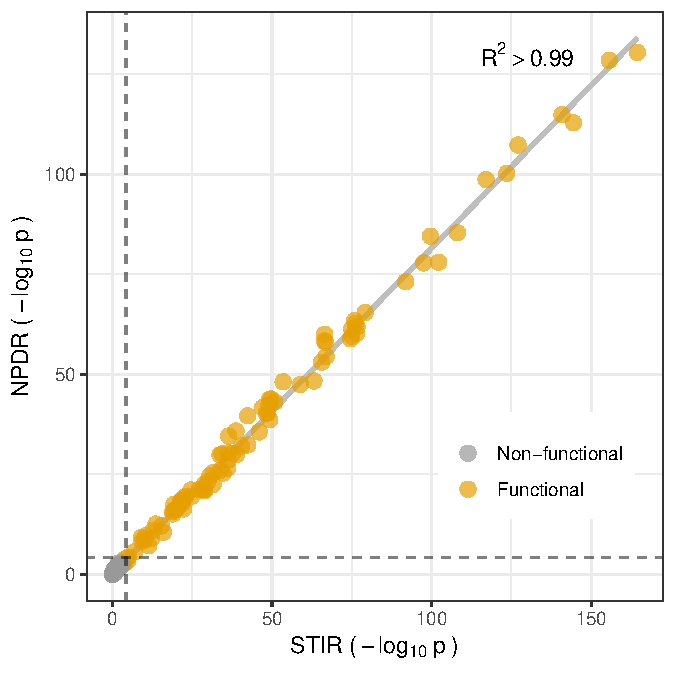
\includegraphics[]{../figs/npdr_stir_p_cc.pdf}}
\caption{\emph{Similarity between NPDR and STIR} in one simulation of $m = 100$ samples and $p = 100$ attributes.}
\label{fig:npdr_stir}
\end{figure}

\begin{figure}[h]%figure2
\centerline{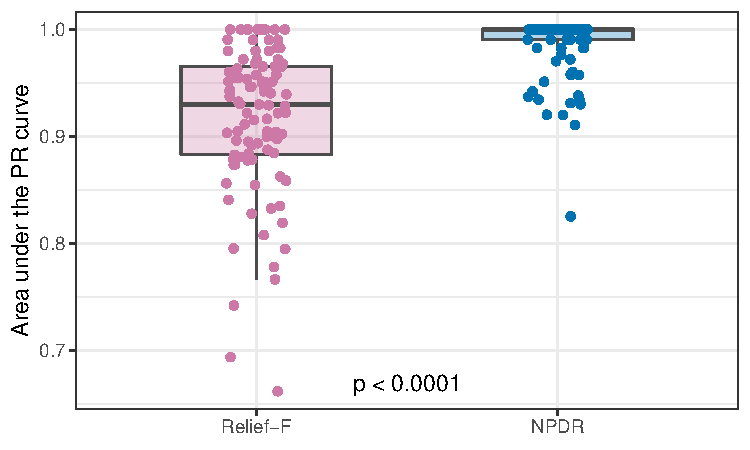
\includegraphics[]{../figs/pr_compare.pdf}}
\caption{\emph{auPRC of Relief-F and NPDR}. Across 100 simulations of $m = 100$ samples and $p = 100$ attributes, NPDR yields significantly higher auPRC.}
\label{fig:auPRC}
\end{figure}



\end{document}
